%!TEX root = ../report.tex
\chapter{Path planning} % (fold)
\label{chap:path_planning}

This chapter covers the path planning algorithm for the robot.
In the first part the trajectory generation process oriented to keep a tarjet in sight is analyzed [\ref{sec:path_planning}]. Then, the constrained planning [\ref{sec:constrained_planning}] is introduced and follows an explanation of the path planner used: RRT-Connect [\ref{sec:path_planning}]. Finally, the implementation [\ref{sec:implementation_pathplanning}], where the constrained planned asumptions and the RRT-Connect parameters are detailed, the experimental results [\ref{sec:experimental_results_pathplanning}] and the conclusions [\ref{sec:conclusions_pathplanning}]of this chapter are presented.

\section{Problem statement} % (fold)
\label{sec:path_planning_in_keep_object_in_sight}
The task considered consists in finding a collision-free trajectory between computed robot configurations so that for every given target position, the tool mounted camera can maintain the marker within its field of view. 
Since the speed of the target has been decided to be kept low for safety reasons, the resulting movement increments of the robot tool are in the order of centimeters. 
This, together with the low quantity of possible obstacles in the workcell where the experiment is carried out, has let the project focus mainly in the constrained planning generation and the path planner utilized.
% section path_planning_in_keep_object_in_view (end)

\section{Constrained planning} % (fold)
\label{sec:constrained_planning}
Hereafter it is assumed that the 3D position of the target is reliably provided to the node.
The input 3D point referred to the reference frame of the camera is first of all, 

*******************************

, for the sake of clarity, lets assume that the object tracked is in the world's reference frame. 
For now, a point in the space is located along with the robot.
The goal is to find a robot configuration that always allows to keep the camera pointing to the tracked object.
Thus, the problem is reduced to find a camera pose that is looking to the object.
This is not trivial due to there are infinite solutions as is going to be shown now. \\

The pose to be found is composed of a vector that defines the position in the space, this is the $x$, $y$ and $z$ coordinates, and the orientation matrix what, in order to clarify the concept, lets assume that this matrix is expressed in the Euler Angles with RPY. So the unknowns of the problem are expressed in a vector of 6 components being this:
******************************

	\begin{equation}
	\label{eq:pose_cartesian_coordinates}
		Pose = [x,y,z,R,P,Y]
	\end{equation}

Under certain assumptions, detailed in the implementation part \ref{sub:contrained_planning_implementation}, the camera pose solutions for a given target position have been reduced from infinite possibilities to a single one. 
Thus, the problem now is to check if the obtained pose is reachable by the robot and yields a collision-free configuration. 
This is made applying inverse kinematics. 
From the possible solutions to the IK problem the most suitable one must be chosen.
The defined one is that which entails the smallest movement of the joints.
% section constrained_planning (end)

\section{Path planning} % (fold)
\label{sec:path_planning}
Once the node computes the desired Q to reach, a single query planner in the configuration space of the robot is used. If the trajectory between initial and goal configurations is detected to be not collision-free, the Rapid-exploring Random Tree RRT in its RRT-Connect variance \cite{RRTConnect} is applied (see figure \ref{fig:rrt_connect}) to find an alternative path.\\

The RRT-Connect is an online algorithm that generates random configurations in the collision free space.
The algorithm used is presented in the listing \ref{lis:rrt_connect_planner} and it defines how from a $q_{init}$ to a $q_{goal}$ $\in$ \ $C_{free}$, a random configuration tree is generated and expanded until the initial and goal configurations are connected. For RRT-Connect to be defined there are some previous factors to be specified. These consist of: metric, collision detector, sampler and the extension.

\begin{lstlisting}[frame=tb, mathescape=true, xleftmargin=.28\textwidth, xrightmargin=.28\textwidth,caption=RRT-Connect Algorithm, label=lis:rrt_connect_planner]
$\textbf{CONNECT}$($\Gamma$, $q$)
 1  repeat 
 2  S $\leftarrow$ EXTEND($\Gamma$,$q$);
 3  until not (S=Advanced)
 4  Return S;
\end{lstlisting}
\lstset{}

\begin{lstlisting}[frame=tb, mathescape=true,xleftmargin=.13\textwidth, xrightmargin=.13\textwidth]
$\textbf{RRT CONNECT PLANNER}$($q_{init}$,$q_{goal}$)
 1  $\Gamma_a$.init($q_{init}$);$\Gamma_b$.init($q_{goal}$);
 2  for k = 1 to K do
 3    q rand $\leftarrow$ RANDOM CONFIG();
 4      if not (EXTEND($\Gamma_a$,$q_{rand}$)=Trapped) then
 5        if (CONNECT($\Gamma_b$,$q_{new}$)=Reached) then
 6        Return PATH($\Gamma_a$,$\Gamma_b$);
 7    SWAP($\Gamma_a$,$\Gamma_b$);
 8  Return Failure
\end{lstlisting}

\begin{figure}[!ht]
	\centering
	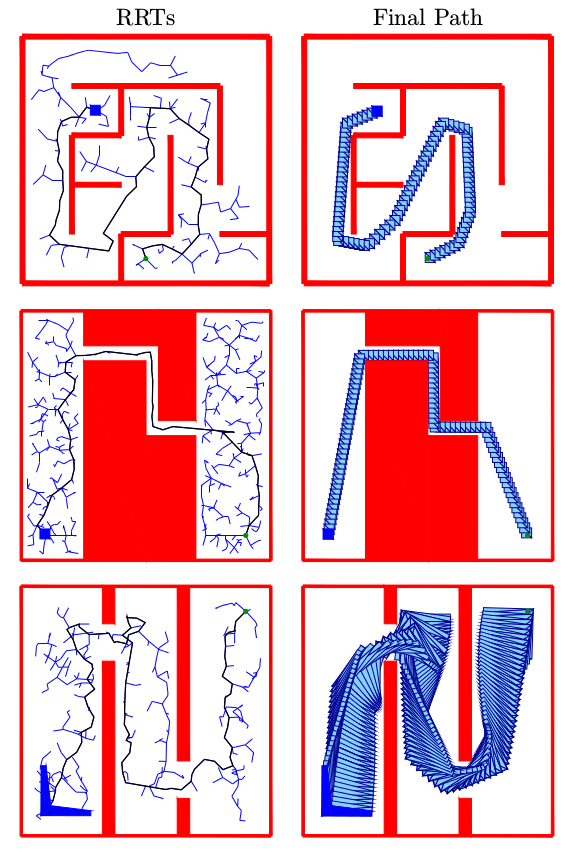
\includegraphics[width=0.4\textwidth]{figures/rrt_connect}
	\caption{RRT-Connect Example}
	\label{fig:rrt_connect}
\end{figure}
% section path_planning (end)

\section{Path optimization} % (fold)
\label{sec:path_optimization}
Due to the speed at which the points are received, the incremental movements of the robot tend to be small, as said above. Therefore, there is little room for path optimization. However given two Q configurations, an interpolation between them is computed.\\

A natural cubic interpolation as the one showed in figure \ref{fig:cubic interpolation}, is carried out. The number of interpolated steps has to be specified so that a higher number means more smoothness but also more path time and lower speed, and vice versa.

\begin{figure}[!hb]
	\centering
	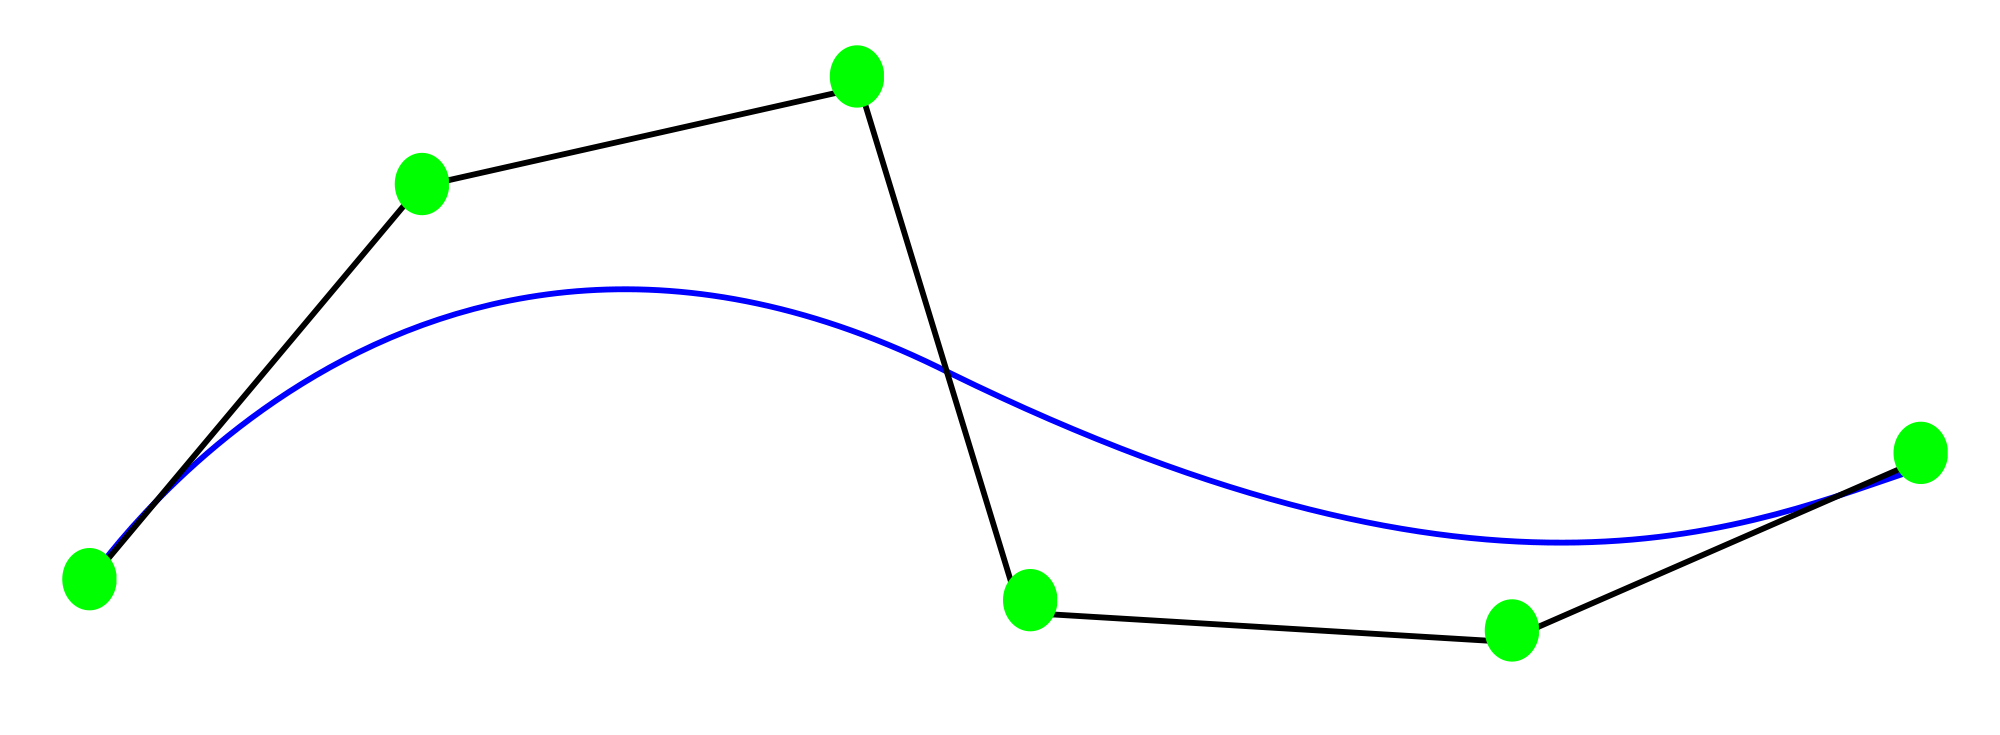
\includegraphics[width=0.8\textwidth]{figures/cubic_interpolation}
	\caption{Cubic interpolation}
	\label{fig:cubic interpolation}
\end{figure}
% section path_optimization (end)

\section{Implementation} % (fold)
\label{sec:implementation_pathplanning}
In the figure \ref{fig:path_planning_flowchart} the flow diagram of this ROS node is showed. The whole node has been developed making use of the ROS and RobWork libraries, and employing the predefined methods offered by them adjusted to best suit the goal.
\begin{figure}[!hb]
	\centering
	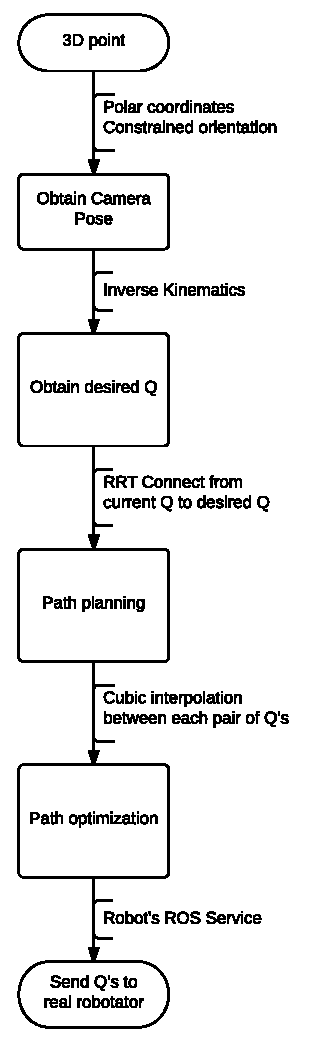
\includegraphics[height=16cm]{figures/path_planning_flowchart}
	\caption{Flowchart of the path planning method}
	\label{fig:path_planning_flowchart}
\end{figure}

	\subsection{Constrained planning} % (fold)
	\label{sub:contrained_planning_implementation}
	\subsubsection{X, Y and Z coordinates} % (fold)
	\label{subsub:x_y_and_z_coordinates}
	To reduce the degrees of freedom of the problem two constraints are applied:
	\begin{enumerate}
		\item The world reference frame is located in the base of the robot.
		\item The camera will keep a fixed distance in the Z axis from the object.
	\end{enumerate}
	The reason for the first assumption is explained later, while the argument for the second is to constrain the problem to a smaller set of solutions. 
	Now, all the possible camera poses lie on the surface of a sphere whose center is the target and whose radius is the specified distance between the camera and the object in Z.
	In order to minimize and control the robot displacement, the most suitable pose has been determined to be that in which the center of the camera belong to the plane formed by the robot's Z base axis and the tracked point. 
	This reduces the set of solutions to the circumference resulting of intersecting the defined plane and the sphere.
	The fact that the robot is now constrained to this plane, makes inverse kinematics solver more likely to find a possible configuration.\\

	So based on the assumption of fixed distance in Z between the target and the camera, a better way to express its pose would be one which includes this distance as a variable.  
	This means that a distance that allows to keep the tracked object far enough to have its whole shape in the image, but close enough for a valid triangulation, must be defined.
	For this reason, and this is only valid when the robot's base is centered in the world reference frame, cylindrical coordinates are used to express the pose vector from \ref{eq:pose_cartesian_coordinates} as in \ref{eq:pose_polar_coorinates};
		\begin{equation}
		\label{eq:pose_polar_coorinates}
			Pose = [r,\alpha,z,R,P,Y]
		\end{equation}
	So transforming the 3D point of the tracked object to cylindrical coordinates it can be obtained the desired pose angle $\alpha$ and the radius $r$ from the robot's base axis. 
	The angle $\alpha$ is the same based on the first assumption and because we want the camera to be in the plane formed by the robot's z base axis and the tracked point. 
	The radius can be calculated as the actual $r_object$ minus the desired distance to the object. Is minus because we want it in the direction of the robot's base. 
	So the camera's pose is now defined as:
		\begin{equation}
		\label{eq:cameras_pose_noRPY_noZ}
			Pose_{camera} = [r_{object},\alpha_{object},z,R,P,Y]
		\end{equation}
	The height keeps being an unknown but, and due to the fact that the next position of the object is unknown, no predictions about the height can be made. 
	For this reason the camera's height is assumed to be the same as the tracked object. This assumption included in the equation \ref{eq:cameras_pose_noRPY_noZ} gives:
		\begin{equation}
			\label{eq:cameras_pose_noRPY}
			Pose_{camera} = [r_{object},\alpha_{object},z_{object},R,P,Y]
		\end{equation}
	% subsection x_y_and_z_coordinates (end)
	\subsubsection{R, P and Y angles} % (fold)
	\label{subsub:r_p_and_y_angles}
	Knowing that the plane ZY of the reference frame of the camera will be contained in the theoretical plane expressed previously, its Z axis must point to the target.

	******************** 

	Assuming that the X and Y axis are parallel to the robot's base frame the angles can be obtained easily.
	This assumption is consistent with the same idea applied in the obtainment of the height. 
	The future state of the object is unknown and due to the robustness of the system is searched, the camera would look directly to the object.\\

	This implies that the camera's Z axis must look to the point, so the roll (R) should be the transformation from the robot's base to the camera plus the angle from the polar coordinates calculated previously.
	Regarding the the pitch (P) and the yaw (Y), is more likely to find a valid state solution if these are parallel to the robot's base reference frame. 
	The camera can be put in another alignment than the base which would include an offset in R,P and/or Y, but supposing the axis are aligned, the final camera's pose is:

	******************************

		\begin{equation}
			\label{eq:cameras_pose}
			Pose_{camera} = [r_{object},\alpha_{object},z_{object},\alpha_{object},0,0]
		\end{equation}
	% subsubsection r_p_and_y_angles (end)
	% subsection contrained_planning (end)

	\subsection{RRT-Connect} % (fold)
	\label{sub:rrt_connect_implementation}
	\subsubsection{Metric} % (fold)
	\label{sub:metric}
	The metric is the way two different robot's configurations are measured. This will define the behavior of the planner along with the extension [\ref{sub:extension}]. For this project, the $Euclidean distance$ has been chosen, due to the balance in the measure that all the joints produce. This is defined by:
	\begin{equation}
		d=\sqrt{\sum_i^N q_i^2}
	\end{equation}
	% subsection metric (end)

	\subsubsection{Extension} % (fold)
	\label{sub:extension}
	The extension is the distance from which another configuration in consider as a neighbor. This distance depends on how the metrics has been defined.
	% subsection extension (end)

	\subsubsection{Collision detector} % (fold)
	\label{sub:collision_detector}
	The collision detector is the strategy used to define when two objects are colliding. Based on our criteria of fast detection and that only simple geometries are found in our work cell, the Yaobi strategy \cite{Yaobi} has been chosen. Yaobi, is defined as a small collision detection library for arbitrary meshes. It is inspired by the libraries PQP and Opcode, and combines a part of both: oriented bounding boxes (OBBs) and hybrid tree structure. Like PQP, Yaobi uses an OBB-tree to model objects. PQP takes this representation to its limit, surrounding each triangle with a single leaf-OBB. Yaobi instead uses the hybrid approach of Opcode, where leaf-nodes surround two triangles each (TriNodes). The hybrid approach not only saves a lot of memory, it also makes collision queries run faster. Benchmarks show that Yaobi is between 2.5 to 3 times faster than PQP. For near convex objects, Opcode is slightly faster, but for curved objects and small objects inside larger ones, Yaobi gets the upper hand.
	% subsection collision_detector (end)
	\subsubsection{Sampler} % (fold)
	\label{sub:sampler}
	The sampler defines how the new configurations need to be created in the $C_{free}$. In this case the sampler chosen has been $Uniform$. This is because of the not patterned geometries so, for example, there is no preference in the direction the new configuration are going to be created.
	% subsection sampler (end)
% subsection rrt_connect (end)
\subsection{Path optimization} % (fold)
\label{sub:path_optimization_implementation}
For the path optimization step some interpolation techniques have been tested. 
From the Circular Interpolator until the Linear Interpolator, the one with best and smoothest results has been the Cubic Spline Interpolator in its natural spline variance.
Due to the fact that the speed of the robot was limited, the factor to define the differential step has been the number of divisions made between two robot configurations. 
During this project a number of 4 intermediate Q's has been used.
% subsection path_optimization (end)


% section implementation (end)

\section{Experimental results} % (fold)
\label{sec:experimental_results_pathplanning}

% section experimental_results (end)

\section{Conclusions} % (fold)
\label{sec:conclusions_pathplanning}
A simple query path planning RRT-Connect, with constrained planning and path optimization has been implemented. \\

On one hand, the assumptions taken when calculating the constrained robot's configuration generation has been proved to be valid for our experiments. 
Furthermore, the RRT-Connect not only has showed to be valid for the project but also has extended our knowledge in this topic, which is inside of the scope of this course.
On the path optimization part, the natural cubic splines have proved to be a good and useful tool when interpolating two Q's, smoothing the robot movements. \\

On the other hand, not only everything has been implemented inside a ROS node and using the RobWork libraries so a further understanding of those has been achieved, but also two auxiliary plugins, the $server point$ and the $Robwork plugin$, has been implemented in parallel so that this node could be tested without depending on the others.

TODO: This is too positive, add some of the experiments conclusions
% section conclusions (end)

% chapter path_planning (end)